\documentclass[tikz,border=2pt,11pt]{standalone}
\usetikzlibrary{arrows.meta}
\usepackage{amsmath}
\usepackage{amssymb}
\usepackage{tikz}
\newcommand{\R}{\mathbb R}
\newcommand{\Z}{\mathbb Z}
\newcommand{\Cyl}{\mathcal C}
\newcommand{\area}{\operatorname{area}}
\newcommand{\dist}{\operatorname{dist}}
\newcommand{\tr}{\operatorname{tr}}
\begin{document}
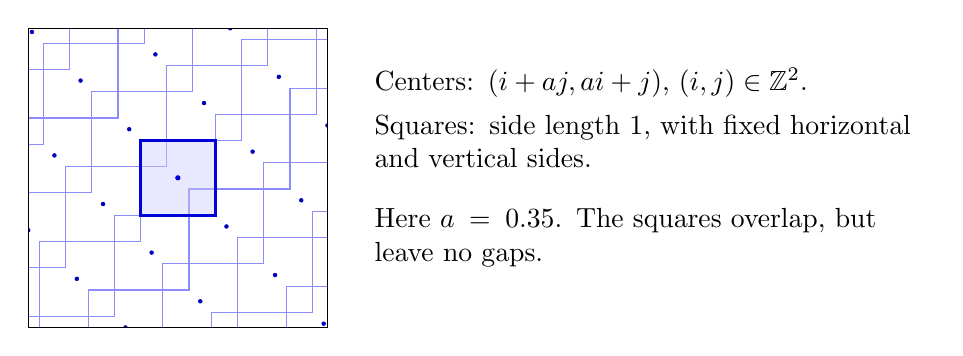
\begin{tikzpicture}[scale=0.95]
 \begin{scope}
  \clip (-2,-2) rectangle (2,2);
  \foreach \i in {-4,...,4} {\foreach \j in {-4,...,4} {
   \pgfmathsetmacro{\cx}{\i+.35*\j}
   \pgfmathsetmacro{\cy}{\j+.35*\i}
   \draw[blue!45,line width=.4pt]
     ({\cx-.5},{\cy-.5}) rectangle ({\cx+.5},{\cy+.5});
   \fill[blue!75!black] (\cx,\cy) circle (.03);
  }}
  \fill[blue!20,opacity=.45] (-.5,-.5) rectangle (.5,.5);
  \draw[blue!85!black,line width=1.1pt] (-.5,-.5) rectangle (.5,.5);
  \fill[blue!85!black] (0,0) circle (.035);
 \end{scope}
 \draw (-2,-2) rectangle (2,2);
 \node[align=left,anchor=west,text width=7cm] at (2.5,.8)
   {Centers: $(i+aj,ai+j)$, $(i,j)\in\Z^2$.\\[4pt]
    Squares: side length $1$, with fixed horizontal and vertical sides.};
 \node[align=left,anchor=west,text width=7cm] at (2.5,-.8)
   {Here $a=0.35$. The squares overlap, but leave no gaps.};
\end{tikzpicture}
\end{document}
